\chapter{Introduction}
\label{sec:intro}

\kant[4] % Dummy text

\section{Figures and Tables}

% Standalone with \input:
\begin{figure}[htbp]
    \centering
    \documentclass[tikz]{standalone}
\begin{document}
    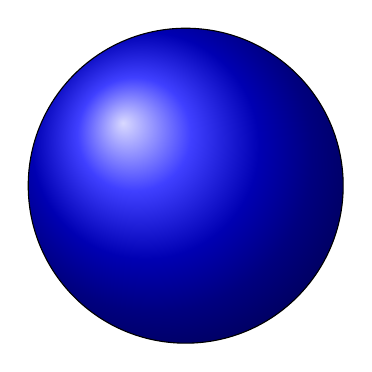
\begin{tikzpicture}
          \draw[shading = ball] (0, 0) circle (2);
    \end{tikzpicture}
\end{document}
    \caption[One ball]{One ball.}
\end{figure}

% Standalone with \includegraphics:
\begin{figure}[thbp]
    \centering
    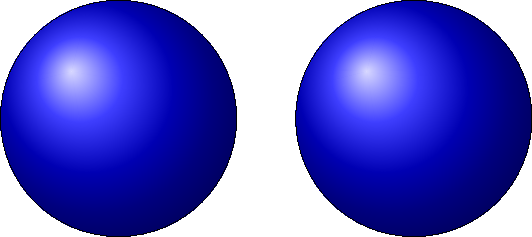
\includegraphics{balls}
    \caption[Two balls]{Two balls.}
\end{figure}

% Todonotes:
\begin{figure}[hbp]
    \centering
    \missingfigure{Three balls.}
    \caption[Three balls]{Three balls.}
\end{figure}

\kant[5-6] % Dummy text

% Booktabs:
\begin{table}[htbp]
    \centering
    \begin{tabular}{cc}
        \toprule
        \textbf{Correct}               & \textbf{Incorrect} \\
        \midrule
        \( \varphi \colon X \to Y \)   & \( \varphi : X \to Y \)  \\[0.5ex]
        \( \varphi(x) \coloneqq x^2 \) & \( \varphi(x) := x^2 \)  \\
        \bottomrule
    \end{tabular}
    \caption[Colons]{Proper colon usage.}
\end{table}

% Tablefootnote and multirow:
\begin{table}[htbp]
    \centering
    \begin{tabular}{cc}
        \toprule
        \textbf{Correct}
        & 
        \textbf{Incorrect}
        \\
        \midrule
        \( -1 \) 
        & 
        -1
        \\[0.3ex]
        1--10
        &
        1-10
        \\[0.3ex]
        Birch--Swinnerton-Dyer\tablefootnote{It is now easy to tell that Birch and Swinnerton-Dyer are two people.} conjecture
        &
        Birch-Swinnerton-Dyer conjecture
        \\[0.3ex]
        The ball \dash which is blue \dash is round.
        &
        \multirow{ 2}{*}{The ball - which is blue - is round.}
        \\[0.3ex]
        The ball---which is blue---is round. 
        &
        \\
        \bottomrule
    \end{tabular}
    \caption[Dashes]{Proper dash usage.}
\end{table}